Il preventivo che regola la suddivisone oraria delle risorse durante le differenti fasi dello sviluppo tiene in considerazione le seguenti quattro regole principali:
\begin{enumerate}
    \item Ogni membro del gruppo deve ricoprire tutti i ruoli di progetto almeno una volta durante lo sviluppo;
    \item Ogni membro del gruppo dovrà sostenere una quantitativo di lavoro totale rendicontato, non superiore alle 105 ore. Viene considerato rendicontato il lavoro svolto in tutte le fasi dello sviluppo eccetto quelle di Analisi e di Analisi di dettaglio, in quanto le ore dedicate per queste fasi sono considerate di investimento non a carico del committente;
    \item Ogni membro del gruppo dovrà sostenere una mole di lavoro comparabile, le ore di lavoro dovranno essere equamente distribuite in ogni fase dello sviluppo;
    \item Non ci devono essere conflitti interessi tra le attività svolte, in nessun caso un verificatore si deve trovare a dover controllare il proprio lavoro svolto all'interno della stessa fase di sviluppo.
\end{enumerate}
Nelle seguenti tabelle verranno utilizzate le seguenti sigle per indicare i vari ruoli:
\begin{itemize}
    \item \textbf{Re}: Responsabile;
    \item \textbf{Am}: Amministratore;
    \item \textbf{Pj}: Progettista;
    \item \textbf{Pr}: Programmatore;
    \item \textbf{Ve}: Verificatore;
    \item \textbf{An}: Analista.
\end{itemize}
Per facilitare la lettura delle tabelle i valori pari a zero, come quantità di ore, sono stati omessi, lasciando uno spazio vuoto.

\newpage
\subsection{Analisi}
\subsubsection{Prospetto orario}
Nella fase di Analisi la distribuzione oraria dei componenti del gruppo, relativamente ai ruoli da loro assunti, è la seguente:

\begin{table}[H]
\taburowcolors[2] 2{tableLineOne .. tableLineTwo}
\tabulinesep = 10pt
\everyrow{\tabucline[.4mm  white]{}}
\begin{tabu} to \textwidth { X[c,4] X[c] X[c] X[c] X[c] X[c] X[c] X[c,2]}
    \tableHeaderStyle
    Nome & Re & Am &  Pj & Pr & Ve & An & Totale \\
    Daniel Mirel Bira &  & 10 &   &  &  & 12 & 22 \\
    Andrea Casagrande &  & 4 &   &  & 12 & 7 & 23 \\
    Fabio Garavello &  & 8 &   &  & 15 &  & 23 \\
    Elena Pontecchiani & 12 & 4 &   &  &  & 7 & 23 \\
    Ilaria Rizzo &  & 3 &   &  & 4 & 15 & 22 \\
    Matteo Squeri & 13 &  &   &  & 7 & 3 & 23 \\
\end{tabu}
\caption{Prospetto orario - Analisi}
\end{table}

Il seguente grafico dà una rappresentazione visiva della suddivisione oraria: 

\begin{figure}[h!]
  \begin{center}
  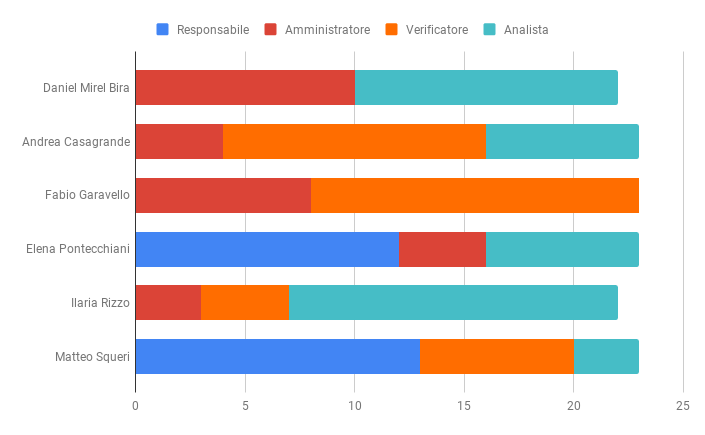
\includegraphics[scale=0.50]{immagini/AnalisiG.png}
  \caption{Grafico suddivisione oraria della fase di Analisi}
  \end{center}
\end{figure}

\newpage
\subsubsection{Prospetto economico}
Nella fase di Analisi la distribuzione delle ore tra i differenti ruoli, con relativo costo, è la seguente:

\begin{table}[H]
\taburowcolors[2] 2{tableLineOne .. tableLineTwo}
\tabulinesep = 10pt
\everyrow{\tabucline[.4mm  white]{}}
\begin{tabu} to \textwidth { X[c] X[c] X[c] }
    \tableHeaderStyle
    Ruolo & Ore & Costo in \euro \\
    Responsabile & 25 & 750,00 \\
    Amministratore & 29 & 580,00 \\
    Progettista &  &  \\
    Programmatore &  &  \\
    Verificatore & 38 & 570,00 \\
    Analista & 44 & 1.100,00 \\
    \textbf{Totale} & \textbf{136} & \textbf{3.000,00} \\
\end{tabu}
\caption{Prospetto economico - Analisi}
\end{table}

Il seguente grafico dà una rappresentazione visiva della suddivisione dei ruoli:

\begin{figure}[h!]
\begin{center}
  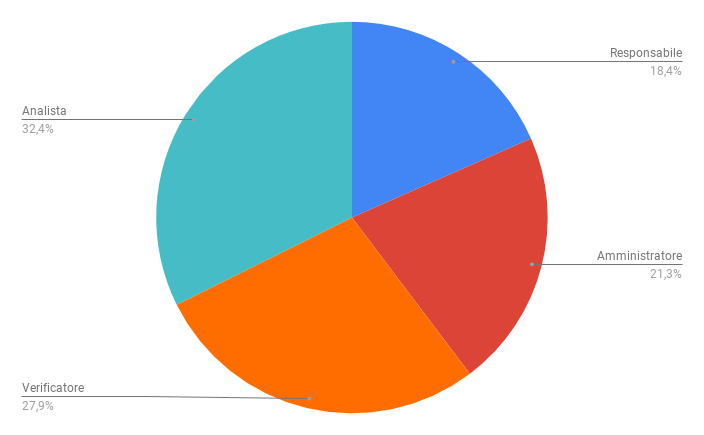
\includegraphics[scale=0.50]{immagini/AnalisiRG.png}
  \caption{Grafico suddivisione dei ruoli della fase di Analisi}
  \end{center}
\end{figure}

\newpage
\subsection{Analisi di dettaglio}
\subsubsection{Prospetto orario}
Nella fase di Analisi di dettaglio la distribuzione oraria dei componenti del gruppo, relativamente ai ruoli da loro assunti, è la seguente:

\begin{table}[H]
\taburowcolors[2] 2{tableLineOne .. tableLineTwo}
\tabulinesep = 10pt
\everyrow{\tabucline[.4mm  white]{}}
\begin{tabu} to \textwidth { X[c,4] X[c] X[c] X[c] X[c] X[c] X[c] X[c,2]}
    \tableHeaderStyle
    Nome & Re & Am &  Pj & Pr & Ve & An & Totale \\
    Daniel Mirel Bira &  &  &   &  & 5 & 3 & 8 \\
    Andrea Casagrande & 7 &  &   &  &  &  & 7 \\
    Fabio Garavello &  & 2 &   &  &  & 6 & 8 \\
    Elena Pontecchiani &  & 4 &   &  &  & 4 & 8 \\
    Ilaria Rizzo &  &  &   &  & 7 &  & 7 \\
    Matteo Squeri &  & 3 &   &  &  & 4 & 7 \\
\end{tabu}
\caption{Prospetto orario - Analisi di dettaglio}
\end{table}

Il seguente grafico dà una rappresentazione visiva della suddivisione oraria:

\begin{figure}[h!]
  \begin{center}
  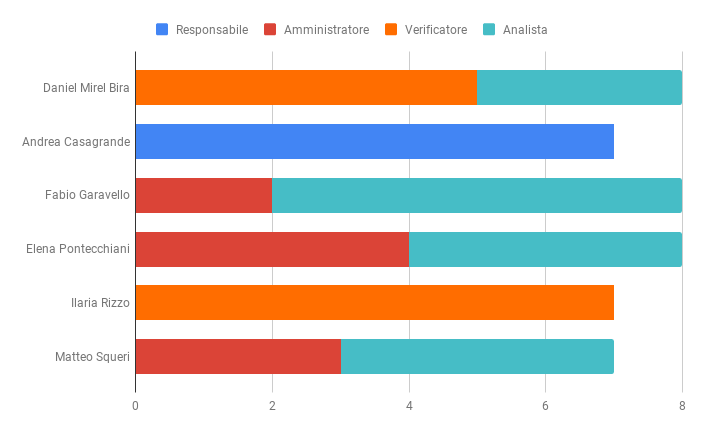
\includegraphics[scale=0.50]{immagini/DettaglioG.png}
  \caption{Grafico suddivisione oraria della fase di Analisi di dettaglio}
  \end{center}
\end{figure}

\newpage
\subsubsection{Prospetto economico}
Nella fase di Analisi di dettaglio la distribuzione delle ore tra i differenti ruoli, con relativo costo, è la seguente:

\begin{table}[H]
\taburowcolors[2] 2{tableLineOne .. tableLineTwo}
\tabulinesep = 10pt
\everyrow{\tabucline[.4mm  white]{}}
\begin{tabu} to \textwidth { X[c] X[c] X[c] }
    \tableHeaderStyle
    Ruolo & Ore & Costo in \euro \\
    Responsabile & 7 & 210,00 \\
    Amministratore & 9 & 180,00 \\
    Progettista &  &  \\
    Programmatore &  &  \\
    Verificatore & 12 & 180,00 \\
    Analista & 17 & 425,00 \\
    \textbf{Totale} & \textbf{45} & \textbf{995,00} \\
\end{tabu}
\caption{Prospetto economico - Analisi di dettaglio}
\end{table}

Il seguente grafico dà una rappresentazione visiva della suddivisione dei ruoli:

\begin{figure}[h!]
  \begin{center}
  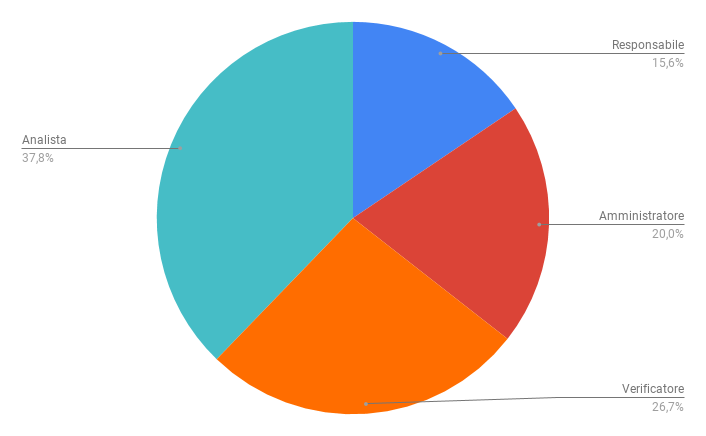
\includegraphics[scale=0.50]{immagini/DettaglioRG.png}
  \caption{Grafico suddivisione dei ruoli della fase di Analisi di dettaglio}
  \end{center}
\end{figure}

\newpage
\subsection{Progettazione della base tecnologica}
\subsubsection{Prospetto orario}
Nella fase di Progettazione della base tecnologica la distribuzione oraria dei componenti del gruppo, relativamente ai ruoli da loro assunti, è la seguente:

\begin{table}[H]
\taburowcolors[2] 2{tableLineOne .. tableLineTwo}
\tabulinesep = 10pt
\everyrow{\tabucline[.4mm  white]{}}
\begin{tabu} to \textwidth { X[c,4] X[c] X[c] X[c] X[c] X[c] X[c] X[c,2]}
    \tableHeaderStyle
    Nome & Re & Am &  Pj & Pr & Ve & An & Totale \\
    Daniel Mirel Bira & 5 &  &   & 18 & 12 &  & 35 \\
    Andrea Casagrande &  & 8 & 15  & 7 & 4 &  & 34 \\
    Fabio Garavello & 5 &  & 6  & 7 & 10 & 7 & 35 \\
    Elena Pontecchiani &  &  & 8  & 8 & 14 & 5 & 35 \\
    Ilaria Rizzo &  & 4 &  10 & 15 & 6 &  & 35 \\
    Matteo Squeri &  &  & 13 & 6 & 5 & 10 & 34 \\
\end{tabu}
\caption{Prospetto orario - Progettazione della base tecnologica}
\end{table}

Il seguente grafico dà una rappresentazione visiva della suddivisione oraria:

\begin{figure}[h!]
  \begin{center}
  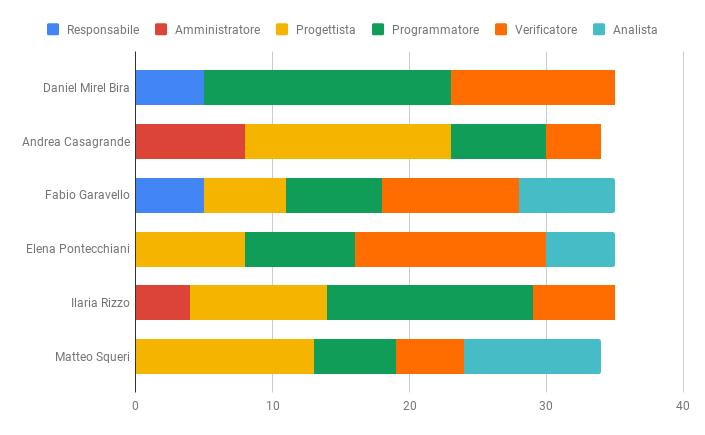
\includegraphics[scale=0.50]{immagini/ProgettazioneG.png}
  \caption{Grafico suddivisione oraria della fase di Progettazione della base tecnologica}
  \end{center}
\end{figure}

\newpage
\subsubsection{Prospetto economico}
Nella fase di Progettazione della base tecnologica la distribuzione delle ore tra i differenti ruoli, con relativo costo, è la seguente:

\begin{table}[H]
\taburowcolors[2] 2{tableLineOne .. tableLineTwo}
\tabulinesep = 10pt
\everyrow{\tabucline[.4mm  white]{}}
\begin{tabu} to \textwidth { X[c] X[c] X[c] }
    \tableHeaderStyle
    Ruolo & Ore & Costo in \euro \\
    Responsabile & 10 & 300,00  \\
    Amministratore & 12 & 240,00 \\
    Progettista & 52 & 1.144,00 \\
    Programmatore & 61 & 915,00 \\
    Verificatore & 51 & 765,00 \\
    Analista & 22 & 550,00 \\
    \textbf{Totale} & \textbf{208} & \textbf{3.914,00} \\
\end{tabu}
\caption{Prospetto economico - Progettazione della base tecnologica}
\end{table}

Il seguente grafico dà una rappresentazione visiva della suddivisione dei ruoli:

\begin{figure}[h!]
  \begin{center}
  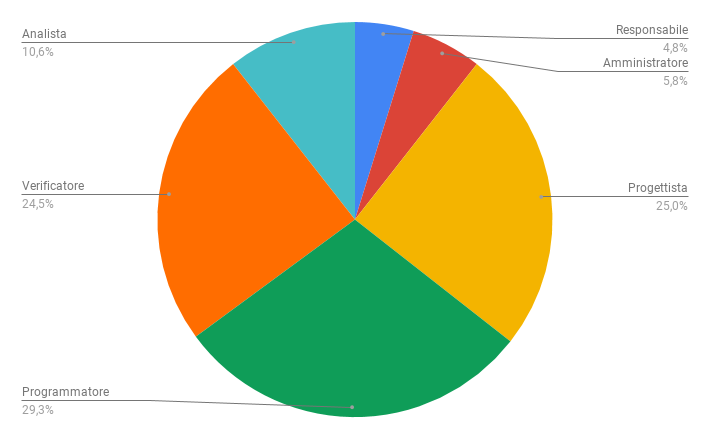
\includegraphics[scale=0.50]{immagini/ProgettazioneRG.png}
  \caption{Grafico suddivisione dei ruoli della fase di Progettazione della base tecnologica}
  \end{center}
\end{figure}

\newpage
\subsection{Progettazione di dettaglio e codifica}
\subsubsection{Prospetto orario}
Nella fase di Progettazione di dettaglio e codifica la distribuzione oraria dei componenti del gruppo, relativamente ai ruoli da loro assunti, è la seguente:

\begin{table}[H]
\taburowcolors[2] 2{tableLineOne .. tableLineTwo}
\tabulinesep = 10pt
\everyrow{\tabucline[.4mm  white]{}}
\begin{tabu} to \textwidth { X[c,4] X[c] X[c] X[c] X[c] X[c] X[c] X[c,2]}
    \tableHeaderStyle
    Nome & Re & Am &  Pj & Pr & Ve & An & Totale \\
    Daniel Mirel Bira &  &  & 20 & 25 &  &  & 45 \\
    Andrea Casagrande &  &  & 13 & 16 & 14 & 2 & 45 \\
    Fabio Garavello &  & 5 &  8 & 15 & 12 & 5 & 45 \\
    Elena Pontecchiani &  & 5 &  12 & 17 & 10  &  & 44  \\
    Ilaria Rizzo & 10 &  &  8 & 18 & 8 &  & 44 \\
    Matteo Squeri & 3 &  & 12 & 20 & 10 &  & 45 \\
\end{tabu}
\caption{Prospetto orario - Progettazione di dettaglio e codifica}
\end{table}

Il seguente grafico dà una rappresentazione visiva della suddivisione oraria:

\begin{figure}[h!]
  \begin{center}
  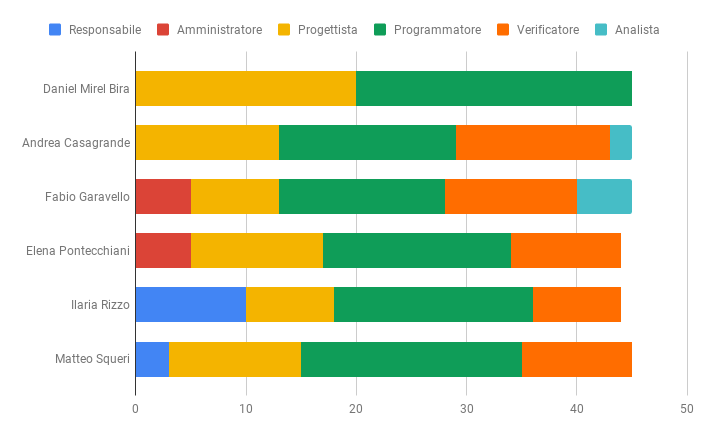
\includegraphics[scale=0.50]{immagini/CodingG.png}
  \caption{Grafico suddivisione oraria della fase di Progettazione di dettaglio e codifica}
  \end{center}
\end{figure}

\newpage
\subsubsection{Prospetto economico}
Nella fase di Progettazione di dettaglio e codifica la distribuzione delle ore tra i differenti ruoli, con relativo costo, è la seguente:

\begin{table}[H]
\taburowcolors[2] 2{tableLineOne .. tableLineTwo}
\tabulinesep = 10pt
\everyrow{\tabucline[.4mm  white]{}}
\begin{tabu} to \textwidth { X[c] X[c] X[c] }
    \tableHeaderStyle
    Ruolo & Ore & Costo in \euro \\
    Responsabile & 13 & 390,00 \\
    Amministratore & 10 & 200,00 \\
    Progettista & 73 & 1.606,00 \\
    Programmatore & 111 & 1.665,00 \\
    Verificatore & 54 & 810,00 \\
    Analista & 7 & 175,00 \\
    \textbf{Totale} & \textbf{268} & \textbf{4.846,00} \\
\end{tabu}
\caption{Prospetto economico - Progettazione di dettaglio e codifica}
\end{table}

Il seguente grafico dà una rappresentazione visiva della suddivisione dei ruoli:

\begin{figure}[h!]
  \begin{center}
  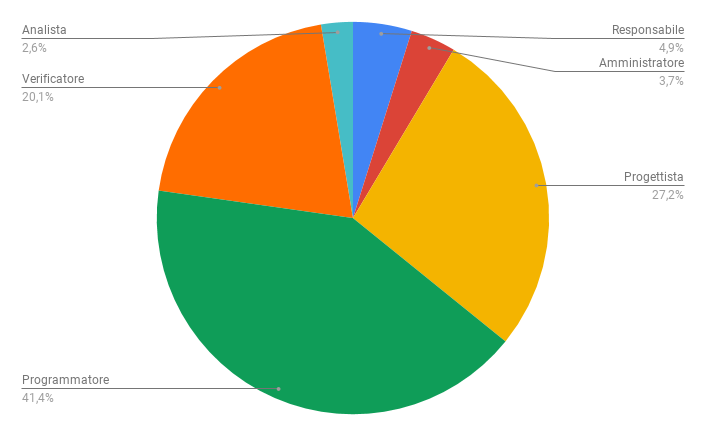
\includegraphics[scale=0.50]{immagini/CodingRG.png}
  \caption{Grafico suddivisione dei ruoli della fase di Progettazione di dettaglio e codifica}
  \end{center}
\end{figure}

\newpage
\subsection{Validazione e collaudo}
\subsubsection{Prospetto orario}
Nella fase di Validazione e collaudo la distribuzione oraria dei componenti del gruppo, relativamente ai ruoli da loro assunti, è la seguente:

\begin{table}[H]
\taburowcolors[2] 2{tableLineOne .. tableLineTwo}
\tabulinesep = 10pt
\everyrow{\tabucline[.4mm  white]{}}
\begin{tabu} to \textwidth { X[c,4] X[c] X[c] X[c] X[c] X[c] X[c] X[c,2]}
    \tableHeaderStyle
    Nome & Re & Am &  Pj & Pr & Ve & An & Totale \\
    Daniel Mirel Bira &  &  &  & 8 & 15 &  & 23 \\
    Andrea Casagrande & 12 & 4 &  &  & 8 &  & 24 \\
    Fabio Garavello &  &  &  10 & 5 & 8 &  & 23 \\
    Elena Pontecchiani &  &  &   & 12 & 12  &  & 24  \\
    Ilaria Rizzo & 4 & 2 & 4 & 10 & 4 &  & 24 \\
    Matteo Squeri &  & 10 & 6 &  & 8 &  & 24\\
\end{tabu}
\caption{Prospetto orario - Validazione e collaudo}
\end{table}

Il seguente grafico dà una rappresentazione visiva della suddivisione oraria:

\begin{figure}[h!]
  \begin{center}
  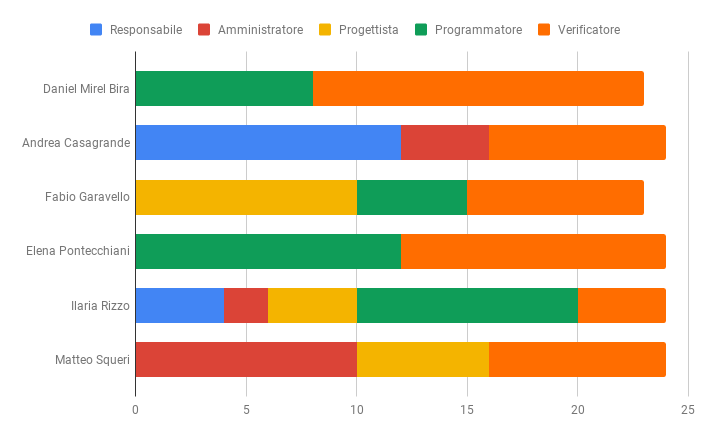
\includegraphics[scale=0.50]{immagini/VerificaG.png}
  \caption{Grafico suddivisione oraria della fase di Validazione e collaudo}
  \end{center}
\end{figure}

\newpage
\subsubsection{Prospetto economico}
Nella fase di Validazione e collaudo la distribuzione delle ore tra i differenti ruoli, con relativo costo, è la seguente:

\begin{table}[H]
\taburowcolors[2] 2{tableLineOne .. tableLineTwo}
\tabulinesep = 10pt
\everyrow{\tabucline[.4mm  white]{}}
\begin{tabu} to \textwidth { X[c] X[c] X[c] }
    \tableHeaderStyle
    Ruolo & Ore & Costo in \euro \\
    Responsabile & 16 & 480,00 \\
    Amministratore & 16  & 320,00 \\
    Progettista & 20 & 440,00 \\
    Programmatore & 35 & 525,00 \\
    Verificatore & 55 & 825,00 \\
    Analista &  &  \\
    \textbf{Totale} & \textbf{142} & \textbf{2.590,00} \\
\end{tabu}
\caption{Prospetto economico - Validazione e collaudo}
\end{table}

Il seguente grafico dà una rappresentazione visiva della suddivisione dei ruoli:

\begin{figure}[h!]
  \begin{center}
  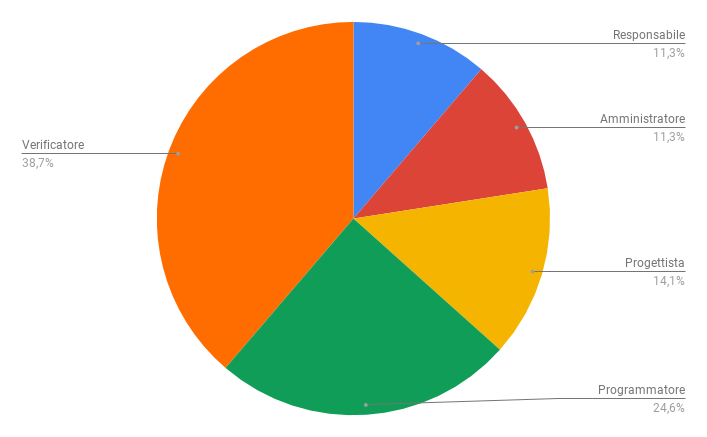
\includegraphics[scale=0.50]{immagini/VerificaRG.png}
  \caption{Grafico suddivisione dei ruoli della fase di Validazione e collaudo}
  \end{center}
\end{figure}

\newpage
\subsection{Totale ore rendicontate}
\subsubsection{Totale suddivisione ore rendicontate}
Sono riportate in questa sezione il totale delle ore di lavoro di ciascun membro del gruppo a carico del \citgl{committente}. Non sono comprese le ore preventivate per le fasi di Analisi e Analisi di dettaglio in quanto considerate di investimento e formazione e quindi non rendicontabili.

\begin{table}[H]
\taburowcolors[2] 2{tableLineOne .. tableLineTwo}
\tabulinesep = 10pt
\everyrow{\tabucline[.4mm  white]{}}
\begin{tabu} to \textwidth { X[c,4] X[c] X[c] X[c] X[c] X[c] X[c] X[c,2]}
    \tableHeaderStyle
    Nome & Re & Am &  Pj & Pr & Ve & An & Totale \\
    Daniel Mirel Bira & 5 &  & 20 & 51 & 27 &  & 103 \\
    Andrea Casagrande & 12 & 12 & 28 & 23 & 26 & 2 & 103 \\
    Fabio Garavello & 5 & 5 & 24 & 27 & 30 & 12 & 103 \\
    Elena Pontecchiani &  & 5 & 20  & 37 & 36  & 5 & 103  \\
    Ilaria Rizzo & 14 & 6 & 22 & 43 & 18 &  & 103 \\
    Matteo Squeri & 3 & 10 & 31 & 26 & 23 & 10 & 103 \\
\end{tabu}
\caption{Totale suddivisione delle ore rendicontate}
\end{table}

Il seguente grafico dà una rappresentazione visiva della suddivisione oraria:

\begin{figure}[h!]
  \begin{center}
  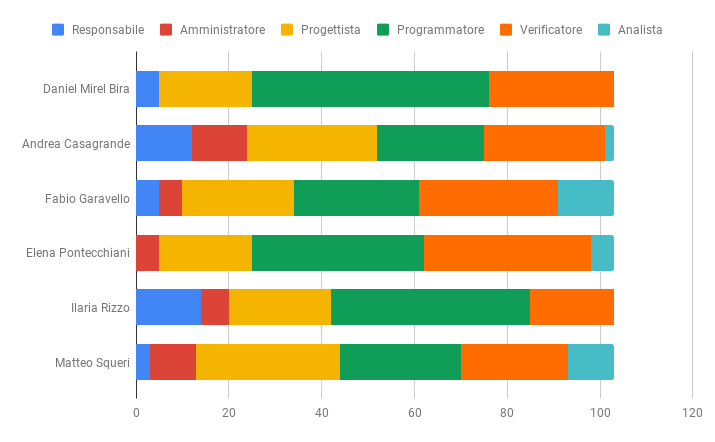
\includegraphics[scale=0.50]{immagini/RendicontateG.png}
  \caption{Grafico della totale suddivisione oraria delle ore rendicontate}
  \end{center}
\end{figure}

\newpage
\subsubsection{Totale del prospetto economico rendicontato}
Sono riportati in questa sezione il costo totale di ogni ruolo, in relazione alle ore in cui sarà attivo, considerando solo le fasi in cui le ore di lavoro sono a carico del committente. Non sono quindi compresi i costi preventivati per le fasi di Analisi e Analisi di dettaglio.

\begin{table}[H]
\taburowcolors[2] 2{tableLineOne .. tableLineTwo}
\tabulinesep = 10pt
\everyrow{\tabucline[.4mm  white]{}}
\begin{tabu} to \textwidth { X[c] X[c] X[c] }
    \tableHeaderStyle
    Ruolo & Ore & Costo in \euro \\
    Responsabile & 39 & 1.170,00 \\
    Amministratore & 38 & 760,00 \\
    Progettista & 145 & 3.190,00 \\
    Programmatore & 207 & 3.105,00 \\
    Verificatore & 160 & 2.400,00 \\
    Analista & 29 & 725,00 \\
    \textbf{Totale} & \textbf{618} & \textbf{11.350,00} \\
\end{tabu}
\caption{Totale del prospetto economico rendicontato}
\end{table}

Il seguente grafico dà una rappresentazione visiva della suddivisione dei ruoli:

\begin{figure}[h!]
  \begin{center}
  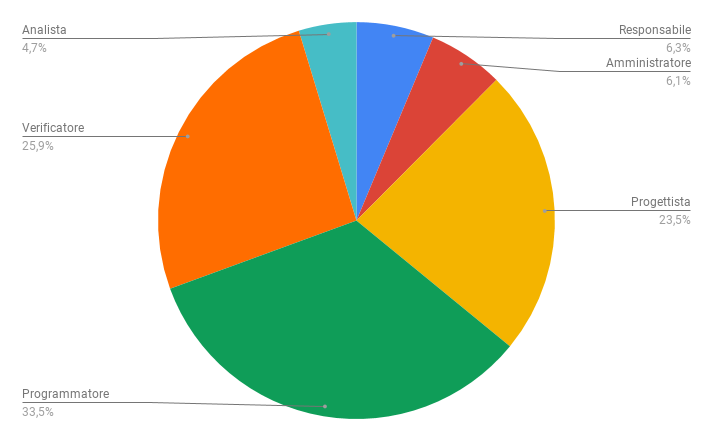
\includegraphics[scale=0.45]{immagini/RendicontateRG.png}
  \caption{Grafico della totale suddivisione dei ruoli delle ore rendicontate}
  \end{center}
\end{figure}

\newpage
\subsection{Totale ore con investimento}
\subsubsection{Totale suddivisione ore con investimento}
Sono riportate in questa sezione il totale delle ore di lavoro preventivate per ciascun membro considerando ogni fase del progetto. 

\begin{table}[H]
\taburowcolors[2] 2{tableLineOne .. tableLineTwo}
\tabulinesep = 10pt
\everyrow{\tabucline[.4mm  white]{}}
\begin{tabu} to \textwidth { X[c,4] X[c] X[c] X[c] X[c] X[c] X[c] X[c,2]}
    \tableHeaderStyle
    Nome & Re & Am &  Pj & Pr & Ve & An & Totale \\
    Daniel Mirel Bira & 5 & 10 & 20 & 51 & 32 & 15 & 133 \\
    Andrea Casagrande & 19 & 16 & 28 & 23 & 38 & 9 & 133 \\
    Fabio Garavello & 5 & 15 & 24 & 27 & 45 & 18 & 134 \\
    Elena Pontecchiani & 12 & 13 & 20 & 37 & 36  & 16 & 134  \\
    Ilaria Rizzo & 14 & 9 & 22 & 43 & 29 & 15 & 132 \\
    Matteo Squeri & 16 & 13 & 31 & 26 & 30 & 17 & 133 \\
\end{tabu}
\caption{Totale suddivisione delle ore con investimento}
\end{table}

Il seguente grafico dà una rappresentazione visiva della suddivisione oraria:

\begin{figure}[h!]
  \begin{center}
  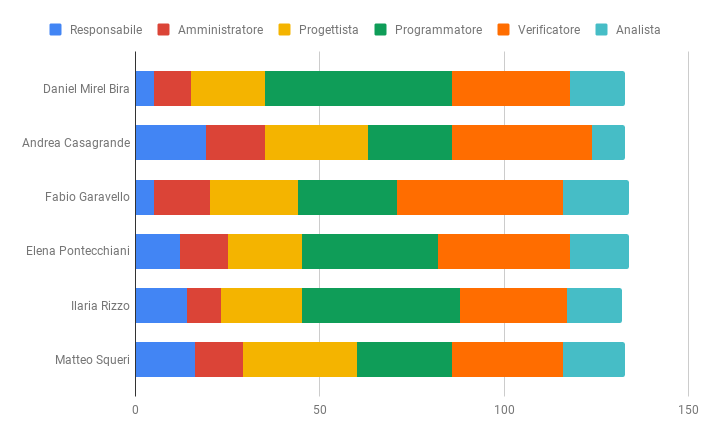
\includegraphics[scale=0.50]{immagini/InvestimentoG.png}
  \caption{Grafico della totale suddivisione oraria delle ore con investimento}
  \end{center}
\end{figure}

\newpage
\subsubsection{Totale del prospetto economico con investimento}
Sono riportati in questa sezione il costo totale di ogni ruolo, in relazione alle ore in cui sarà attivo, considerando ogni fase del progetto.

\begin{table}[H]
\taburowcolors[2] 2{tableLineOne .. tableLineTwo}
\tabulinesep = 10pt
\everyrow{\tabucline[.4mm  white]{}}
\begin{tabu} to \textwidth { X[c] X[c] X[c] }
    \tableHeaderStyle
    Ruolo & Ore & Costo in \euro \\
    Responsabile & 71 & 2.130,00 \\
    Amministratore & 76 & 1.520,00 \\
    Progettista & 145 & 3.190,00 \\
    Programmatore & 207 & 3.105,00 \\
    Verificatore & 210 & 3.150,00 \\
    Analista & 90 & 2.250,00 \\
    \textbf{Totale} & \textbf{799} & \textbf{15.345,00} \\
\end{tabu}
\caption{Totale del prospetto economico con investimento}
\end{table}

Il seguente grafico dà una rappresentazione visiva della suddivisione dei ruoli:

\begin{figure}[h!]
  \begin{center}
  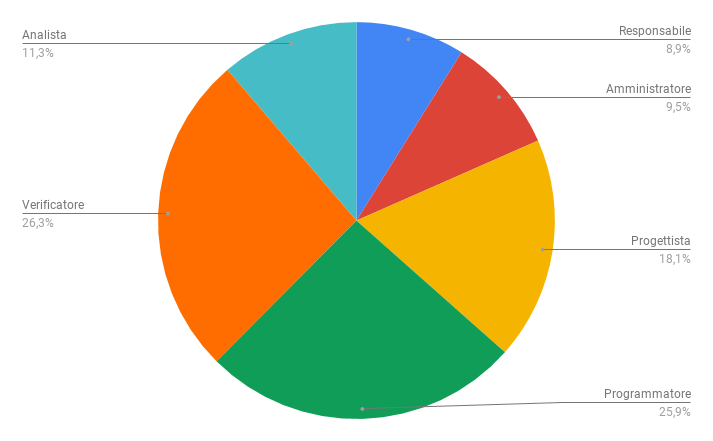
\includegraphics[scale=0.45]{immagini/InvestimentoRG.png}
  \caption{Grafico della totale suddivisione dei ruoli delle ore con investimento}
  \end{center}
\end{figure}